\documentclass[10pt]{article}
\usepackage{geometry}
\geometry{letterpaper}           % ... or a4paper or a5paper or ... 
%\geometry{landscape}            % Activate for for rotated page geometry
\usepackage[parfill]{parskip}    % Activate to begin paragraphs with an empty line rather than an indent
\usepackage{graphicx}
\usepackage{amssymb}
\usepackage{epstopdf}
\DeclareGraphicsRule{.tif}{png}{.png}{`convert #1 `dirname #1`/`basename #1 .tif`.png}
\usepackage{hyperref}
\usepackage{amsmath}

\title{Notes on building a classifier for SAT instances}
\author{A bunch of smart people{\footnote{Including the author}}}

\begin{document}
\maketitle
We want to understand what makes certain SAT instances harder to solve than the
others. Let's assume we are given a bunch of metrics that characterize SAT
instances. What do you do? You can ask how you got those parameteres, i.e., are
they natural? Or you could ask how well those parameters work in classifying
the instances. Further, you may also ask which of these parameters contribute
most to the classification. These notes are about systematically addressing the questions
after the ``Or''.

\section{How well do the parameters work for classifying the instances?}
We have 512 parameters, and two features that we want to predict: solving time
(a continuous variable) and a category (verification, agile, crypto, crafted
and random).

\subsection{Classifying into category of instances}
Here, we want to solve the following problem: given a new SAT instance, can we
predict which category of instance it belongs to? Perhaps a more nuanced
question to ask would be which category is the formula "closest" to. This,
however, requires a metric, and in the absence of one, we are going to compute
distances using a Euclideian metric.    

\subsubsection{Visualizing the data}
What if we could see some data points are closer to each other than others,
i.e., see that the data naturally forms classses?  Our data lives in a 512
dimensional space. Good luck visualizing this. A really cool technique used by
data scientists is called t-SNE (short for t-distributed Stochastic Neighbour embedding). 
\textit{It converts similarities between data points to joint probabilities and
tries to minimize the Kullback-Leibler divergence between the joint
probabilities of the low-dimensional embedding and the high-dimensional data.
t-SNE has a cost function that is not convex, i.e. with different
initializations we can get different results.} Therefore, one needs to be careful while
interpreting t-SNE plots. Here are some laws-of-the-land~\cite{wattenberg2016how}.
\begin{enumerate}
    \item Hyperparameters matter. 
    \item Cluster sizes in a t-SNE plot mean nothing. 
    \item Distances between clusters might not mean anything.
    \item Random noise doesn’t always look random. 
\end{enumerate}

\begin{figure}[h]
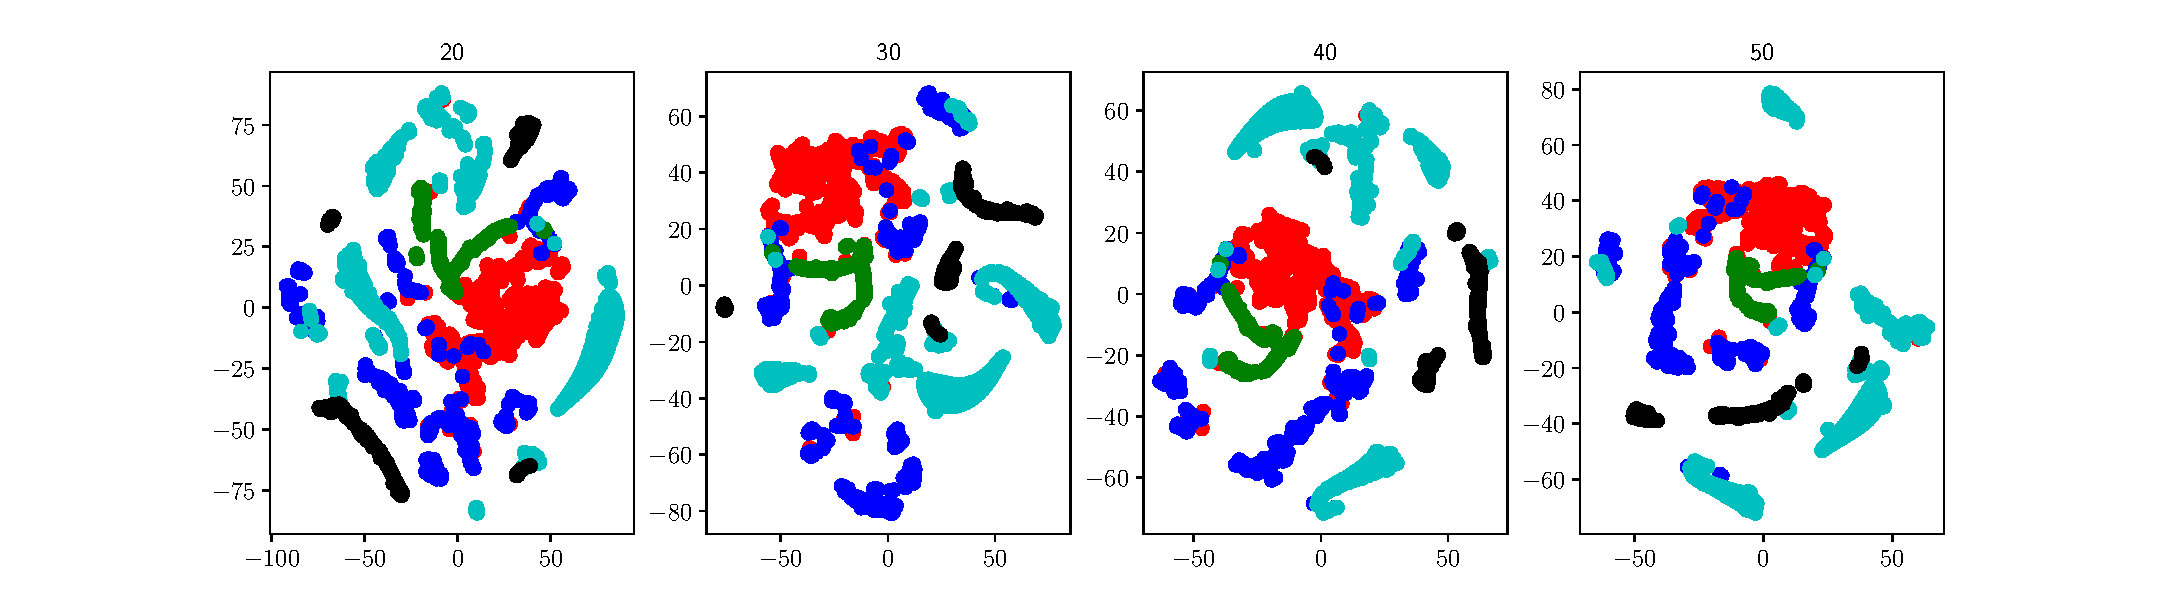
\includegraphics[width=\linewidth]{tSNE/Category.pdf}
\caption{t-SNE plot for categories of Instances. Each plot corresponds to a
different value of perplexiety (one of the hyperparameters) for 1000 iterations
(the other hyperparameter). The colour coding is as follows: verification
(red), agile (blue), crypto (green), crafted (cyan),  random (black). We can
identify clusters in the data independent of the hyperparameters.}
\end{figure}

\subsubsection{Building a classifier}
We now show the results of several classification algorithms (cause we don't
really know the theory behind each one to have a favourite).

\begin{table}
\begin{center}
\renewcommand{\arraystretch}{1.2}
\begin{tabular}{ l  c  c }
 \label{tab:MNIST}
 Classifier & Accuracy & $2\sigma$ \\
 \hline
  \texttt{KNeighborsClassifier(nneighbors=3)} & 0.94 & 0.23 \\
  \texttt{SVC(C=0.025, kernel='linear')} & 0.94  & 0.20 \\
  \texttt{SVC(C=1, gamma=2)} & 0.92 & 0.23 \\
  \texttt{DecisionTreeClassifier(maxdepth=5)} & 0.93 & 0.22 \\
  \texttt{RandomForestClassifier(maxdepth=5, maxfeatures=1, nestimators=10)} & 0.94 & 0.19 \\
  \texttt{MLPClassifier(alpha=1, maxiter=1000)} & 0.94 & 0.20 \\
  \texttt{AdaBoostClassifier()} & 0.55 & 0.09 \\
  \texttt{GaussianNB()} & 0.83 & 0.15
\end{tabular}
\caption{Classifier results for category classification.}
\end{center}
\end{table}

However, what do these numbers mean? We do have good accuracy, but our
$2\sigma$ bounds are really large. For comparison, let's look at how these same
classifiers behave on MNIST dataset. See table~\ref{tab:MNIST}.

\begin{table}
\begin{center}
\renewcommand{\arraystretch}{1.2}
\begin{tabular}{ l  c  c }
 \label{tab:MNIST}
 Classifier & Accuracy & $2\sigma$ \\
 \hline
  \texttt{KNeighborsClassifier(nneighbors=3)} & 0.98 & 0.03 \\
  \texttt{SVC(C=0.025, kernel='linear')} & 0.96  & 0.04 \\
  \texttt{SVC(C=1, gamma=2)} & 0.12 & 0.06 \\
  \texttt{DecisionTreeClassifier(maxdepth=5)} & 0.64 & 0.09 \\
  \texttt{RandomForestClassifier(maxdepth=5, maxfeatures=1, nestimators=10)} & 0.80 & 0.12 \\
  \texttt{MLPClassifier(alpha=1, maxiter=1000)} & 0.95 & 0.06 \\
  \texttt{AdaBoostClassifier()} & 0.26 & 0.07 \\
  \texttt{GaussianNB()} & 0.81 & 0.13
\end{tabular}
\caption{Classifier results for MNIST dataset.}
\end{center}
\end{table}


\subsection{Classifying into hard and easy}
\subsubsection{Visualizations}
Similar to what we did for understanding the clustering for Category, we visualize
how the clustering reflects hardness. We classify hardness as follows. 
\begin{equation}
    \label{eq:HardnessLabel}
    H(t) = \{\mathrm{Hard, if~}t > 60 \mathrm{;~else, Easy} \},
\end{equation}
where $t$ is the solving time measured in seconds.  
\begin{figure}[h]
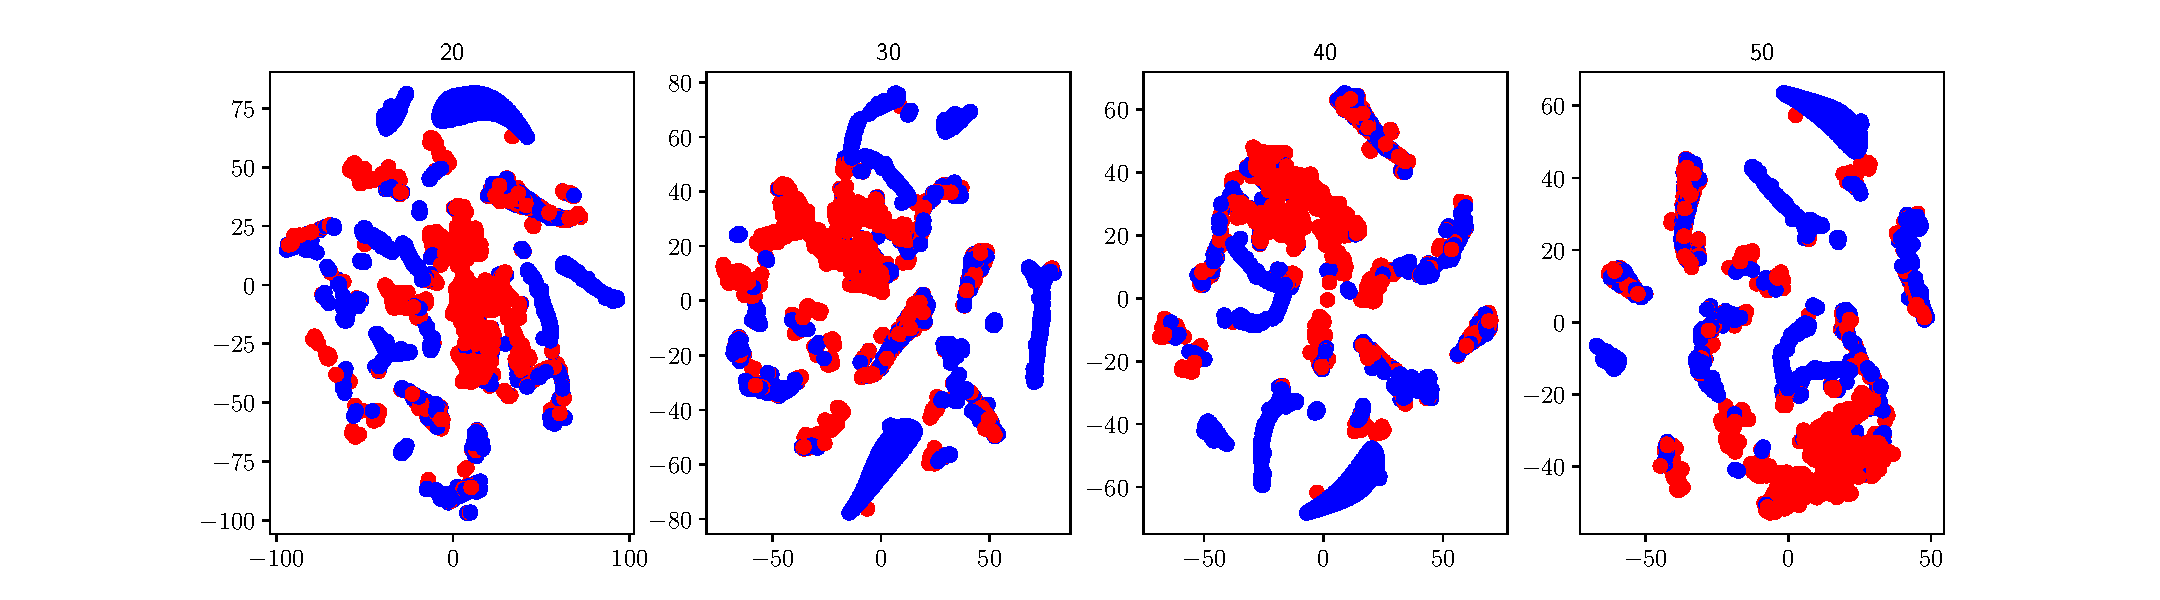
\includegraphics[width=\linewidth]{tSNE/Hardness.pdf}
\caption{t-SNE plot for hardness with all categories considered together. Red
corresponds to Easy instances and blue corresponds to the Hard instances
defined according to Eq.~(\ref{eq:HardnessLabel})}
\end{figure}
We can also ask how separable easy and hard instances are in each individual
category; see Fig.~(\ref{fig:Verification}--\ref{fig:Random})   
\begin{figure}[h]
    \label{fig:Verification}
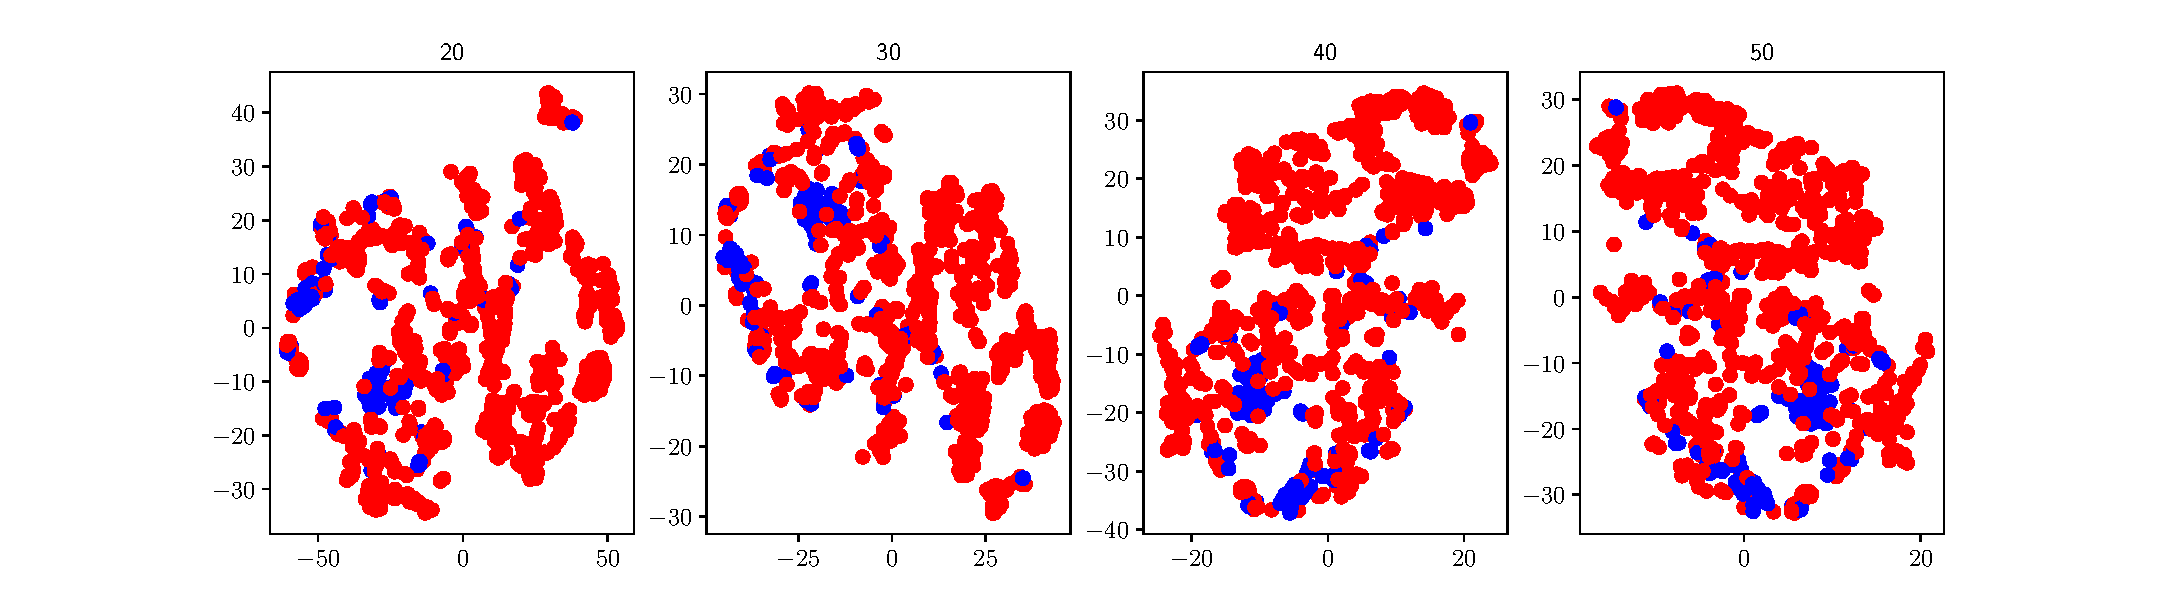
\includegraphics[width=\linewidth]{tSNE/Hardness_Verification.pdf}
\caption{Verification}
\end{figure}
\begin{figure}[h]
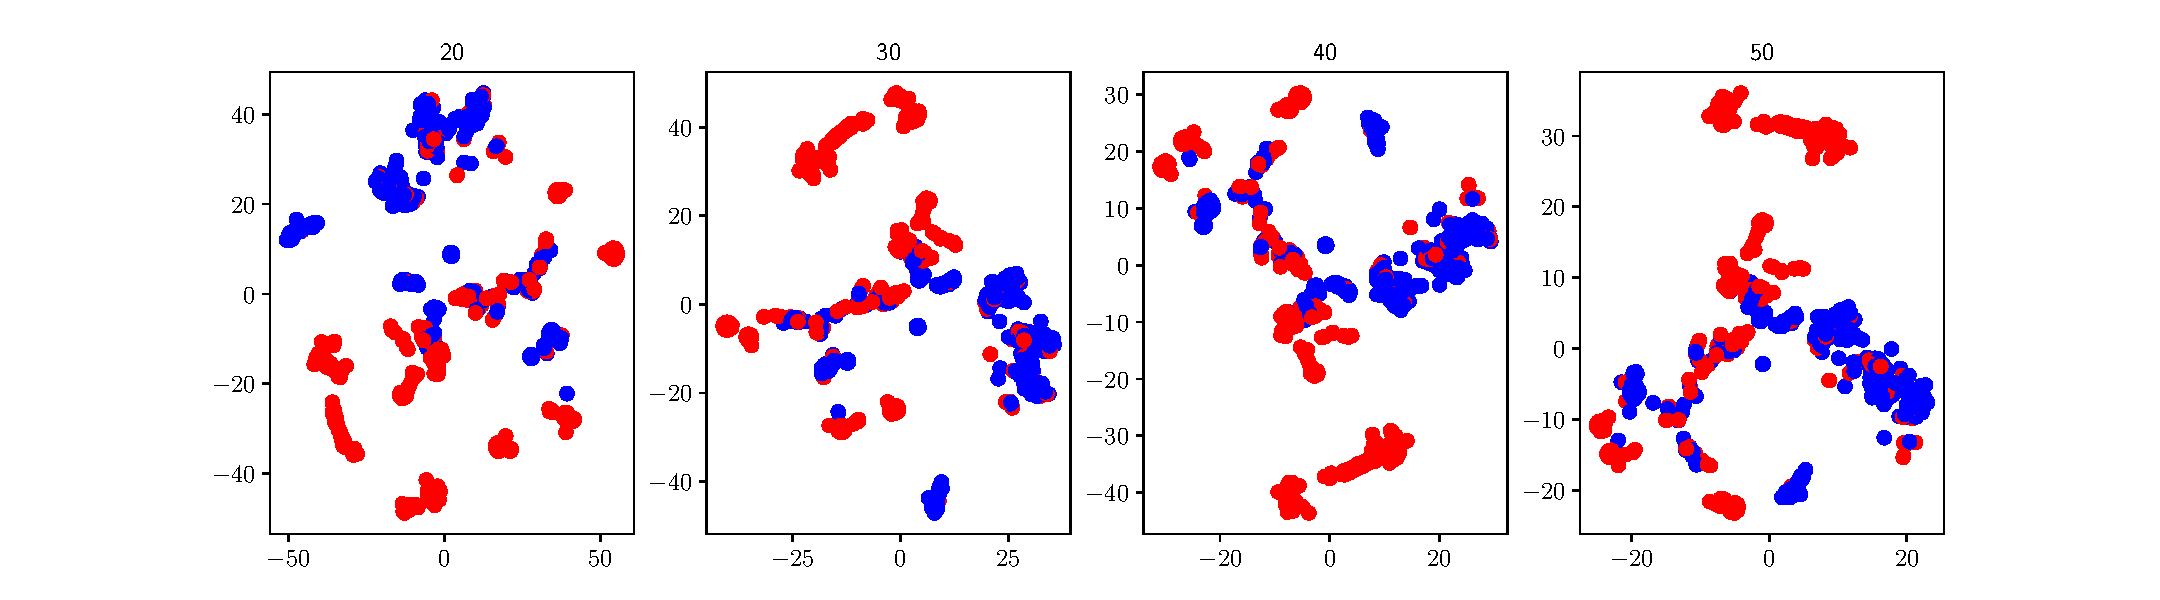
\includegraphics[width=\linewidth]{tSNE/Hardness_Agile.pdf}
\caption{Agile}
\end{figure}
\begin{figure}[h]
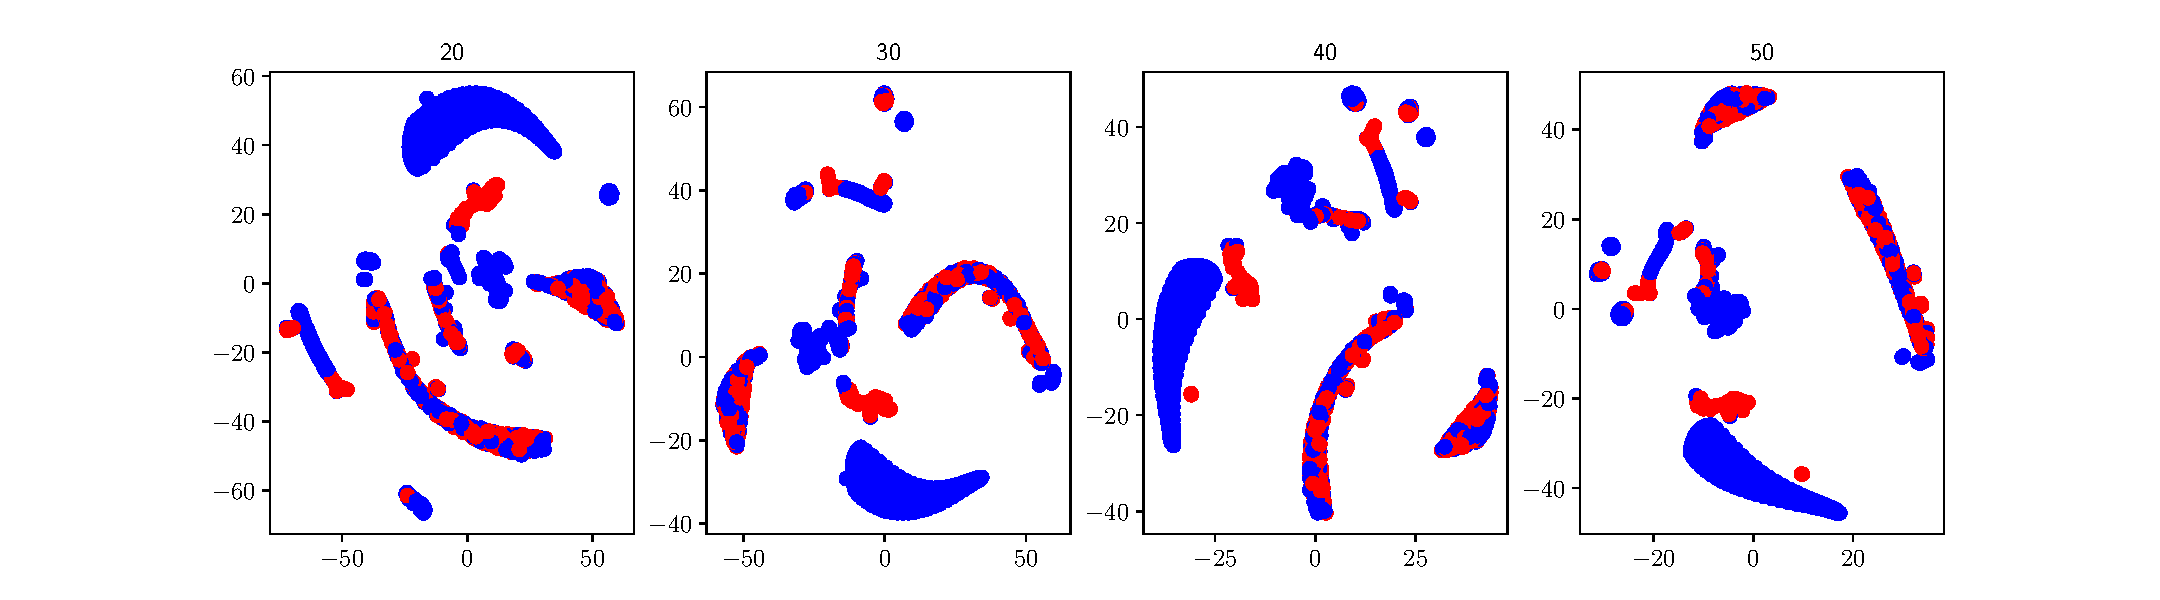
\includegraphics[width=\linewidth]{tSNE/Hardness_Crafted.pdf}
\caption{Crafted}
\end{figure}
\begin{figure}[h]
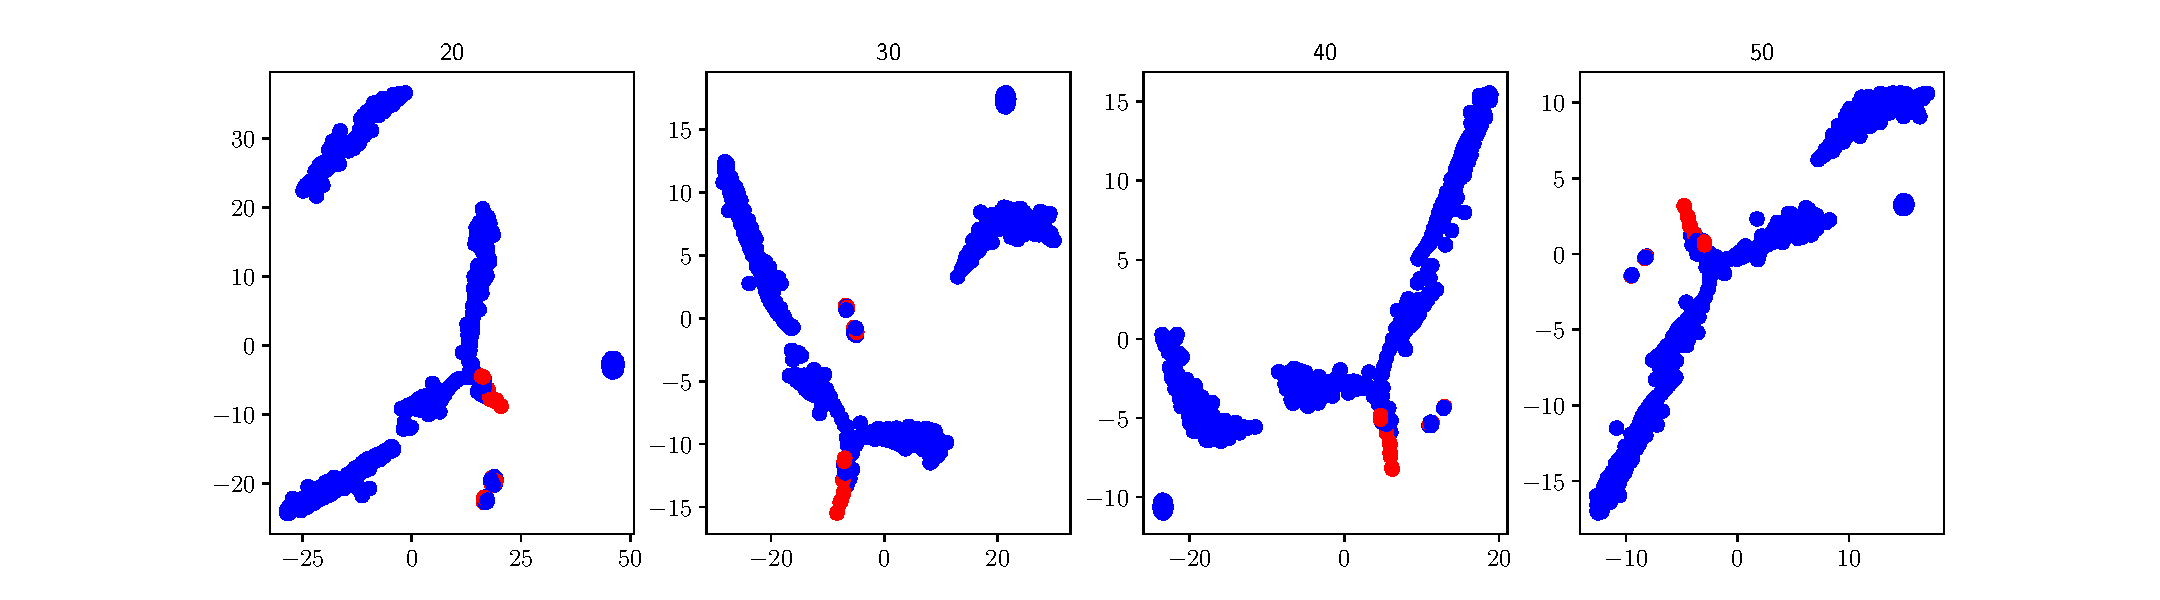
\includegraphics[width=\linewidth]{tSNE/Hardness_Crypto.pdf}
\caption{Crypto}
\end{figure}
\begin{figure}[h]
    \label{fig:Random}
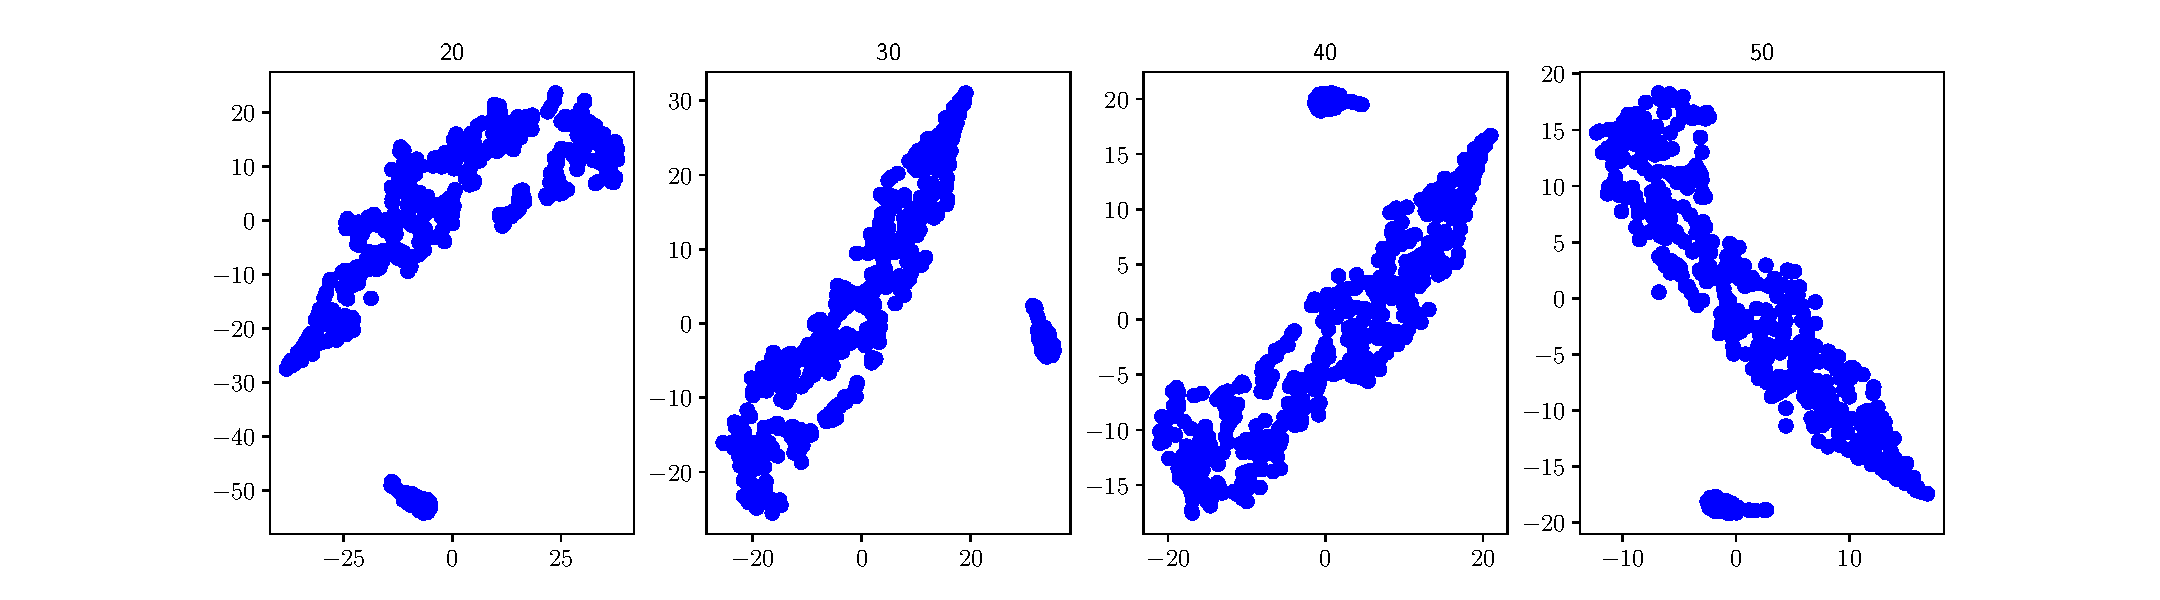
\includegraphics[width=\linewidth]{tSNE/Hardness_Random.pdf}
\caption{Random}
\end{figure}

\subsubsection{Classifying hardness}
\begin{table}[h]
\begin{center}
\renewcommand{\arraystretch}{1.2}
\begin{tabular}{ l  c  c }
 \label{tab:MNIST}
 Classifier & Accuracy & $2\sigma$ \\
 \hline
  \texttt{KNeighborsClassifier(nneighbors=3)} & 0.74 & 0.30 \\
  \texttt{SVC(C=0.025, kernel='linear')} & 0.61  & 0.23 \\
  \texttt{SVC(C=1, gamma=2)} & 0.74 & 0.32 \\
  \texttt{DecisionTreeClassifier(maxdepth=5)} & 0.71 & 0.31 \\
  \texttt{RandomForestClassifier(maxdepth=5, maxfeatures=1, nestimators=10)} & 0.76 & 0.30 \\
  \texttt{MLPClassifier(alpha=1, maxiter=1000)} & 0.69 & 0.28 \\
  \texttt{AdaBoostClassifier()} & 0.75 & 0.30 \\
  \texttt{GaussianNB()} & 0.66 & 0.23
\end{tabular}
\caption{Classifier results for hardness classification.}
\end{center}
\end{table}

\section{Which are the most important parameters in the classification?}





\bibliographystyle{unsrt}
\bibliography{soham-notes}
\end{document}  
